\documentclass{article}

% \usepackage[utf8]{inputenc} %Stationær ÆØÅ
% \usepackage[ansinew]{inputenc} %Bærbar ÆØÅ?

\usepackage{amsthm} %Eksamples
\usepackage{pgfgantt} %Package for gantcharts
\usepackage{hyperref} % Allows in document hyperrefs
%\usepackage{url} % Allows hyperlinks
\usepackage{minted} % In document sourcecode
% \usepackage[hyphens]{url} %URLs
% \usepackage{graphicx} % Allows figures
\usepackage{etoolbox} %for configuration of sloppy
% \usepackage{tabularx} %Tabulars
%Section style
\usepackage{xcolor}
\usepackage{minted}

\usepackage{tikz}
\tikzstyle{class} = [
    rectangle, 
    rounded corners, 
    fill=black!40,
    % shading=axis,
    % bottom color =black!20,
    top color = white,
    % top color    =white,
    % shading angle=45,
    draw, 
    minimum size=5mm
    ]

\definecolor{secnum}{RGB}{102,102,102}

\makeatletter
    \def\@seccntformat#1{\llap{\color{secnum}\csname the#1\endcsname\hskip 16pt}}
\makeatother
%end section style

{\sloppy}{\hbadness 10000\relax}{}{} %adds hbadness to sloppy
\setlength{\paperheight}{297mm} %Sets the page to an A4
\setlength{\paperwidth}{210mm}        %Sets the page to an A4

%macros
\newcommand{\HF}{\texttt{HIPERFIT}}
\newcommand{\HQL}{\texttt{HQL}}
\newcommand{\QL}{\texttt{QuantLib}}
\newcommand{\Cpp}{\texttt{C++}}

%example
\theoremstyle{definition}
\newtheorem{exmp}{Example}[section]

%Ganttchart
\definecolor{stblue}{RGB}{0,253,155}
\definecolor{stred}{RGB}{234,87,0}

\newganttchartelement{stbar}{
    stbar/.style={ 
      shape=rounded rectangle,
      inner sep=0pt,
      draw=stblue!50!black,
      very thick,
      top color=white,
      bottom color=stblue!50
    },
    stbar incomplete/.style={
        /pgfgantt/stbar,
        draw=stred,
        bottom color=stred!50
    },
    stbar label font=\slshape,
    % stbar left shift=-.1,
    % stbar right shift=.1
}

\begin{document}

\begin{titlepage}
\begin{center}
\textsc{\huge Haskell Library for Quantitative Analysis in Finance}\\[0.5cm]
% \textsc{\Large Midway Report}\\[0.5cm]
\vspace{2 cm}
\begin{tabular}{ll}
Student: & Kasper Passov\\
Supervisors: & Fritz Henglein \\ 
             & Jost Berthold
\end{tabular}
\end{center}
\vspace{5 cm}
\newpage
\tableofcontents
\end{titlepage}

\section{Problem Description}

\section{Problem Definition}

I want to design and develop a Haskell library for 
quantitative finance, taking the open source \QL\ 
as a starting point. The language Haskell is used
because of its purity and advanced type class system
which allows it to model relevant entities.\\
The result of my project should be a software
architecture that supports different kinds of 
financial instruments and valuation methods.

\section{Learning Goals}
The following are the goals i hope to fulfill during this project:
\begin{itemize}
    \item {I will be able to work with models of different financial instruments and pricing methods.}
    \item {I will be able to structure and execute a medium-sized software project in a functional language.}
    \item {I will be able to implement parts of a medium-sized financial project using Haskell.}
    \item {I will be able to use advanced Haskell typesystem features.}
\end{itemize}
Overall i hope to gain a deeper knowledge of Haskell and functional programming, an overview of the basic finacial instruments
and methods and gain experience in structuring and completing a sizeable project.

\section{Project Specifications}
The project will be an extension of the Haskell library \HQL, implementing 
some of the functionality of the \Cpp\ library \QL\cite{QULI}, onto the current system.\\
The \QL\ library is writen in object oriented programming style (\Cpp) and uses a class system, 
which is not strictly translateable into the Haskell type class system.
Haskell type classes ensures that some operations will be availabe for values of chosen types, meaning they are
more similar to abstract classes with multiple inheritance, such as the \texttt{Java Interface}, 
than with the actual \Cpp\ classes. \\
This raises the problem of a class architecture that cannot be directly translatet, as a \Cpp\ class cannot translate
into a Haskell type class. I will analyse and extract the architecture of \QL\ and redesign it to accomodate
the new type class system, without removing functionality.\\
The main milestone of the project is to implement the vanilla swap functionality into the
current \HQL\ library. This will have several hurdles, as a vanilla swap is a swap of a fixed interest
rate with a floating rate. At the time of writing, floating interest rate is not implemented in \HQL, so 
another part of the project would entail the addition of this functionality. \\

\section{Project Limitations}
As \QL\ is a large library, implementing everything would be a much to large task
for a bachelor project, meaning only parts of the \QL\ functionality will be added to \HQL.\\
As statet above, the main milestone of the project is the implementation of vanilla swaps, and
all dependant functionality. After the milestone is reached, further analysis 
of \QL\ will be done, resulting in selection and prioritisation of more expansions to the \HQL\ library.
I will however ignore date calculations in my implementation as this broadens the scope beyond what is 
possible of this project. 

\section{Project Justification}

\subsection{Justification of a Quantitative Library}
The field of Quantitative analysis is calling for evermore computational power, to
do the calculations needed for the exponetialy expanding data volumes, using the 
computation-intesive methods for complex risk analysis.\\
The context my project will take base on is the quantitative library \HQL\cite{HQL},
developed within the \HF\cite{HF} research center, by master students Andreas Bock 
and Johan Astborg supervised by Jost Berthold and Sinan Gabel. 
The library is one in a chain of projects made by \HF, striving to develop 
functional programming solutions designed for highly parallel computation architectures.
Making it easier to implement massive parallelization into (among others) financial 
methods and instruments\cite{FHPH}.

\subsection{Language Justification}
Andreas Bock and Johan Astborg was given the language Haskell for development of \HQL\cite{HQL},
(as part of \HF s general goal of creating financialy highlevel functional programing tools\cite{HF}). 
As my project is based on \HQL, the justification of the language is largely the same, and i will paraphase their reasoning.\\
The correctness of the program is paramount in the development of a quantitative library, as 
the finance sector is very suspectible to faulty software, where even small errors
can lead to large economical damage. Because of this, we wish our language capable
of catching as many errors as possible in the compilation phase. \\
In this Haskell excels, as its strict type system allows us to eliminate any type errors during compilation
whereas \Cpp, some of these errors might first be found in runtime.
Furthermore Haskell has a number of attractive features making it suited
for financial calculations, including modularity\cite{WFM}, laziness\cite{Cc}, functionality, purity and type classes.\\
The purity makes it easier to translate equations into code because of maths inherent purity,
and as different financial products often shares similar functionality, the functional 
programming of Haskell enables us to re-use code or create new functionality from existing one.
Haskell allows overloading functionality based on types using type classes, this is extremely desirable
as it allows us to have the same API regardless of exact type (e.g. an \texttt{Instrument} can be used abstractly 
as a parameter, so functions can have different functionality based on the exact instance of \texttt{Instrument}).

\section{Problem Analysis}

\subsection{Financial Concepts}

\subsubsection{Terminology}
\paragraph{Maturity}
The maturity refers to the finite time period in which a financial instrument
exists, at the end of maturity the principal is repaid with interest. 

\paragraph{Principal}
The principal of a loan is the amount of money invested in this loan, separated from interest. 
\paragraph{Basis point}
A basis point is one-hundredth of a 1\%, and is commonly used for calculating
changes in interest\cite{InvOp}. So a 50 basic point change of interest would be a change of either $+0.5\%$ or $-0.5\%$.
\paragraph{LIBOR}
The London Interbank Offered Rate, or LIBOR, is the worlds most commonly used reference for floating-rate interest. It is the rate at which
banks can borrow funds from other banks in the London interbank market. From a banks point of view, this is the rate at which they will
lend or borrow money from each other, for various maturities\cite{LIBOR}.\\ 
The LIBOR rate is calculated everyday after 11:00 (UK Time) on behaf of the British Bankers' Association\cite{LIBORInfo},
and is published in 8 maturities and 5 currencies\cite{LIBORRate}. In 2013 the BBA discontinued 5 other currencies, including the swedish and danish crown, and 
8 maturities\cite{LIBORDisc}. \\
\paragraph{Long and Short position}
Taking a long position is buying a stock, commodity or currency with the expectation that the asset will rise in value.
Taking a short position is borrowing with the expectation that the asset will fall in value\cite{InvOp}.
\subsubsection{Swaps}
John C.Hull defines a swap as an over-the-counter agreement between two companies to exchange cashflows in the future\cite{BOG}[Chap 7.].
The most common form of swap is the \emph{plain vanillaswap} interest rate swap. In this swap, a companie agree to pay a fixed rate
cashflow of a determined principal for a determined number of years. The reciever then pays a floating rate interest of the same principal
in the same timeframe. These two cashflows are called respectively the Fixed Leg and the Floating Leg of the vanillaswap.
One common use of the swaps, is to transform the nature of an asset. 
An example of using swap to transform a liability as taken from John C.Hull\cite{BOG}.
\begin{exmp}
    Company A has an outgoing cashflow on a floating-rate loan of LIBOR plus 0.1\% on a principal of \$100 million, that it wants to transform
    into a fixed-rate loan. 
    % Company B wishes to transform a fixed-rate loan of 5\% with the same principal into a floating-rate loan, so they enter into a vanillaswap agreement. 
    Company B agrees to enter into the swap, thus they loan each other \$100 million with company A paying a fixed-rate of 5.0\% to company B
    and company B paying a floating rate of LIBOR to company A.\\
    Company A has the following three sets of cash flows, after the swap has been entered: 
    \begin{enumerate}
        \item It pays LIBOR plus 0.5 to the outside lender\%.
        \item It recieves a LIBOR floating-rate from B.
        \item It pays a 5.0\% fixed-rate to B.
    \end{enumerate}
    This nets company A a fixed-rate interest payment of 5.5\%, instead of the floating-rate LIBOR + 0.5\%, this is illustrated on figure \ref{fig:swapTrans}.
\end{exmp}

\begin{figure}[h]
    \centering
    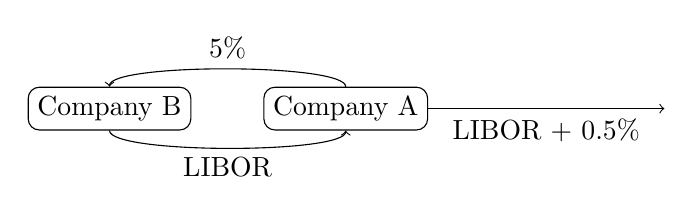
\begin{tikzpicture}[node distance=2cm]
        \node (A) [class] at (0,0) {Company A}; 

        \node (B) [class] at (-3,0) {Company B}; 

        % Lines
        \draw[->] (A.north) .. controls +(up:3mm) and +(up:3mm) .. node[above] {5\%} (B.north);
        \draw[->] (B.south) .. controls +(down:3mm) and +(down:3mm) .. node[below] {LIBOR} (A.south);
        \draw[->] (A.east) -- node[below] {LIBOR + 0.5\%} ++ (3,0);

    \end{tikzpicture}
    \caption{Using swaps to transform a liability}
    \label{fig:swapTrans}
\end{figure}

\subsubsection{Valuation of Swaps}

Things to explain.\\
Cashflow Coupons, Fixed, basic points, Instrument, Swaps, VanillaSwap\\
% Options(?)



\section{Architecture Design}
\subsection{Analysis}
Detailing previous analysis of c++ architecture.\\

\subsection{Implementation}
Theory behind Model/Instrument/Pricing Engine, and remodeling of existing HQL splitting
the Model and Instrument into seperat entities.\\
Justification of class hirachies (split them so future additions such as Commodities and Dividents
can be added onto the system easily).


\subsubsection{Cashflow}
Like in QuantLib i would like to create a hierachy of classes where the 
most general class holds as much functionality as possible. For the legs
of our Swap, we would like to have a floating leg and a fixed leg. These
can be described as Coupons, or even more generaly, as Cashflows. 
In QuantLib the Cashflow base interface contains among others, a method
to return the amount of a Cashflow. The Quantlib Cashflow class also contains
methods regarding the dates of the Cashflow, and a hook, this is not modeled
in HQL as of this work. 

\begin{minted}{haskell}
class Cashflow a where 
    amount :: a -> Double        
\end{minted}

\subsubsection{Coupons}
Inherents from Cashflow.
accrued rate, returning the interest rate accrued by the coupon.
dayCounter, daycount convention.
accrued ammount, takes a date and returns the accrued amount of cash from the Coupon until the given date.
Wrap these in a monad or disregard them?

\begin{minted}{haskell}
class Cashflow a => Coupon a where
    rate :: a -> Rate
\end{minted}

\subsubsection{Fixed and Floating Rate Coupon}
Instances of Coupons.
More work in swap to find out exacly what methods are needed.

\begin{minted}{haskell}
data FixedRateCoupon = FixedRateCoupon Rate -- InterestRate?
instance Coupon FixedRateCoupon where
  rate (FixedRateCoupon r) = r 
\end{minted}
Something interesting on the implementation. Possibly the usage
of typefamilies to allow Continuously and Simple Rate with little
extra code. 

\subsubsection{Swaps}
More hirachy and inheretence.
Description of the chosen functionality and implementation of it.
\begin{minted}{haskell}
class Instrument s => Swap s where
  -- | returns whenever the swap is expired
  isExpired :: s -> bool
  -- | startdate of the swap
  startDate :: s -> Date 
  -- | calculates the maturity date of the swap
  maturityDate :: s -> Date
  -- | calculates the net present value of the swap 
  legNPV :: s -> Double 
  -- | calculates the basis point of the swap
  legBPS :: s -> Double 
\end{minted}
Maybe use a multiparameterclass here

\subsubsection{VanillaSwaps}
Description of the chosen functionality and implementation of it.
\begin{minted}{haskell}
data VanillaSwap = VanillaSwap FixedRateCoupon FloatingRateCoupon
\end{minted}

\begin{thebibliography}{9}
\bibitem{OOSE}
    Bernd Bruegge, Allen H.Dutoit
    \emph{Object-Oriented Software Engineering Using UML, Patterns and Java},
    Person New International Edition,
    Third Edition,
    2014.
\bibitem{QULI}
    Luigi Ballabio
    \emph{Implementing \QL},
    Draft,
    2013.
\bibitem{HQL}
    Andreas Bock, johan Astborg, Jost Berthold, Sinan Gabel
    \emph{HIPERFIT Quant Library},
    2014.
\bibitem{WFM}
    John Hughes, The University Glasgow
    \emph{Why Functional Programming Matters} 
    1990.
\bibitem{Cc}
    Simon Peyton Jones, Jean-Marc Eber, Julian Seward
    \emph{Composing contracts: an adventure in financial engineering}
    2000.
\bibitem{HF}
    http://hiperfit.dk/
\bibitem{FHPH}
    Jost Berthold, Andrzej Filinski, Fritz Henglein, Ken Friis Larsen, Mogens Steffensen, Brian Vinter
    \emph{Functional High Performance Financial IT}
    2012.
\bibitem{BOG}
    John C.Hull
    \emph{Options, Futures, and other Derivatives}
    Eight edition
\bibitem{InvOp}
    http://www.investopedia.com/dictionary/
\bibitem{LIBOR}
    \emph{London Interbank Offered Rate}
    www.stat.unc.edu/faculty/cji/fys/2010/LIBOR.pdf
\bibitem{LIBORInfo}
    LIBOR definition
    www.global-rates.com/interest-rates/libor/libor-information.aspx
\bibitem{LIBORRate}
    LIBOR Rates
    www.global-rates.com/interest-rates/libor/libor.aspx.
\bibitem{LIBORDisc}
    LIBOR Discontinued
    www.global-rates.com/interest-rates/libor/libor.aspx
\end{thebibliography}

\end{document}

